\documentclass{article}
\usepackage{amsmath,amssymb}
\usepackage{bm}
\usepackage[numbers,sort&compress]{natbib}
\usepackage{color}
\usepackage{graphicx}

\newcommand{\Ca}{\mathrm{Ca}}
\newcommand{\beq}{\begin{equation}}
\newcommand{\feq}{\end{equation}}
\newcommand{\beqal}{\begin{equation}\begin{aligned}}
\newcommand{\feqal}{\end{aligned}\end{equation}}

\title{Conditions for successful wetting during collision between emulsion droplets and curved substrate}
\begin{document}
\maketitle
\section{Abstract}
\section{introduction}
Emulsion droplets are often used a delivery vehicle to deposit active ingredients on target substrates in application such as drug delivery, cosmetics and detergent products. In order to fulfill their function emulsion formulation are optimized in terms of emulsion droplets size, stability, surface properties and interaction forces with the target substrate. Virtually the properties of the emulsion droplets while stored before their use and their behavior after wetting the target substrate can be finely designed using well established physical models that identify the critical parameters controlling stability and adhesion properties.

However, to fulfill its function, the emulsion droplets need to be successfully transferred on the substrate. This transfer process, that involves the complex sequence of events that take the emulsion droplets from the formulated state to the substrate is not as well characterized and the role of the different parameters related to the emulsion, substrate and hydrodynamic interaction mediated by the continuous phase is still poorly defined. Recent AFM studied of emulsion interactions identified the critical role of hydrodynamic effect on the repulsion between two emulsions colliding at different speed. The effective disjointing pressure preventing contact and coalescence between the two emulsion droplets has an electrostatic and an hydrodynamic component. This suggest that also during the process of emulsion collision on a substrate successful contact and wetting of the surface critically depend on the interplay of the hydrodynamic and inter-facial properties. 

In this work we use Lattice Boltzmann simulation methods to study the effect of inter-facial and hydrodynamic parameters on the efficiency of the wetting process during collision. We simulate a spherical emulsion droplets colliding on a curved "cylindrical" substrate. The properties of the substrate are set by controlling its curvature and the three phase contact angle with the emulsion droplet and the surrounding fluid. The emulsion droplet is characterized by its size, viscosity and inter-facial tension with the surrounding fluid. The hydrodynamic properties are explored by simulating droplet collision on the substrate under different flow conditions. 

In the Next section we describe the idealized collision system simulated, the physical properties controlled in the simulation and the range of parameters explored (parameter space). In the following section we provide details about the simulation methods and its validation against other methodology previously proposed (Binary-liquid lattice Boltzmann model). Next we summarize the results of the parametric study focusing on the behavior of the emulsion as it collides with the substrate as a function of the interfacial and hydrodinamic parameters explored (Results). We then propose a map of the deposition efficiency within the explored parametric space (deposition efficiency map). Finally we summarize the results and relate to the related application areas (conclusions). 
 
\section{parameter space}
 
\section{Binary-liquid lattice Boltzmann model}
The lattice Boltzmann equation (LBE) operates on a rectangular grid representing the
physical domain. It utilizes
probability distribution functions (also known as particle populations)
containing information about
macroscopic variables, such as fluid density, momentum, and the phase order parameter for multiphase models. LBE consists of
two parts: a local collision step, and a propagation step which transports
information from one node to another along some 
directions specified by the discrete velocity set.
The LBE is typically implemented as follows:
\begin{equation}
\label{standard:implementation}
\begin{aligned}
&f_i^{*}(\bm{x},t)=\omega f_i^{eq}(\bm{x},t)-(1-\omega) f_i(\bm{x},t) +
F_i,&&\text{ collision step}\\
&f_i(\bm{x}+\bm{c_i},t+1)=f_i^{*}(\bm{x},t),&&\text{ propagation step}, 
\end{aligned}
\end{equation}
where $f_i$ is the probability distribution function in the direction $\bm{c_i}$,
 $f_i^{eq}$ is the equilibrium probability distribution function, $\omega$ is the
relaxation parameter, and $F_i$ is the external force population. The force population
represents an external physical force and is implemented in the current work using the scheme
outlined in \citet{guo}.

The binary fluid LB model is
based on a free-energy functional \cite{swift,landau}, and operates with two
sets of populations: one to track the pressure and the velocity fields, and another to represent the
phase field $\phi$ indicating the gas or liquid.

The model we use is a two-dimensional nine-velocity (D2Q9) model,
with equilibrium populations \cite{pooley-contact}:
\begin{equation}
\label{set:equilibrium:binary}
\begin{aligned}
&f_i^{eq}&&=w_i 
\biggl(3
p_0 - k \phi \Delta \phi
+\rho\frac{u_{\alpha}c_{i\alpha}}{c_s^2}+\rho \frac{Q_{i\alpha\beta}u_{\alpha } u_ {
\beta}}{2 c_s^4}\biggr)\\
&&&+k\bigl(w_i^{xx} (\partial_x \phi)^2+w_i^{yy} (\partial_y \phi)^2 +w_i^{xy} \partial_x
\phi \partial_y \phi \bigr), 1\leq i \leq 8\\
&f_0^{eq}&&=\rho-\sum_{i\neq0}{f_i^{eq}}\\
&g_i^{eq}&&=w_i\left(\Gamma \mu + \phi\frac{ c_{i\alpha} u_{i\alpha}}{c_s^2}+\phi
\frac{Q_{i\alpha\beta}u_{\alpha}u_{\beta}}{2 c_s^4}\right), 1\leq i \leq 8 \\
&g_0^{eq}&&=\phi-\sum_{i\neq0}{g_i^{eq}}\quad,
\end{aligned}
\end{equation}
where $\Gamma$ is the mobility parameter; the chemical potential
$\mu=-A\phi+A\phi^3-k\Delta\phi$; $k$ is the parameter related to the surface
tension; $A$ is the parameter of the free-energy model. The bulk pressure
is expressed as $p_0=c_s^2 \rho +A (-0.5 \phi^2+0.75 \phi^4)$ with
the sound speed $c_s^2=1/3$. 
Parameters specific to the D2Q9 grid are the weights
$w_i=\left\{\frac{4}{9},\frac{1}{9},\frac{1}{9},\frac{1}{9},\frac{1}{9},
\frac{1}{36},\frac{1}{36},\frac{1}{36},\frac{1}{36}\right\}$, and the tensor
$Q_{i\alpha\beta}=c_{i\alpha} c_{i\beta} - c_s^2 \delta_{\alpha\beta}$.  
Other weights 
are as follows:
$w^{xx}_{1-2}=w^{yy}_{3-4}=1/3$, $w^{xx}_{3-4}=w^{yy}_{1-2}=-1/6$,
$w^{xx}_{5-8}=w^{yy}_{5-8}=-1/24$, $w^{xy}_{1-4}=0$, $w^{xy}_{5-6}=1/4$ and
$w^{xy}_{7-8}=-1/4$. 

One can show that the set of discrete evolution equations (\ref{set:equilibrium:binary}) restores the
macroscopic
multiphase equations through the Chapman-Enskog analysis \cite{chapman}:
\begin{equation}
\begin{aligned}
&\partial_t \rho+ \partial_{\alpha} \rho u_{\alpha}=0\\
&\rho\left(\partial_t+u_{\beta}\partial_{\beta}\right) u_{\alpha}= F_{\alpha}
-\partial_{\beta}P_{\alpha \beta} +
\nu\partial_{\beta}\left(\partial_{\alpha}u_{\beta}+\partial_{\beta} u_{\alpha}\right)\\
&\partial_t \phi + \partial_{\alpha} \phi u_{\alpha}=M \partial^2_{\beta\beta} \mu,
\end{aligned}
\label{binary:fluid:system}
\end{equation}
where $\nu=c_s^2 (\tau-1/2)$ is the viscosity,
$M=\Gamma(\tau_{\phi}-1/2)$ is the mobility parameter, and $\tau=\frac{1}{\omega}$ and $\tau_{\phi}$
are the relaxation parameters of density and phase fields, 
$P_{\alpha\beta}=\Bigl(p_0-k\phi \Delta \phi -\frac{k}{2}|\nabla \phi|^2\Bigr)\delta_{\alpha\beta}
+ k \partial_{\alpha} \phi \partial_{\beta} \phi$  \cite{pooley-contact}.The interface tension value
in the framework of the binary liquid model is $\gamma=\sqrt{\frac{8 k
A}{9}}$. The inclusion of the interface tension in the momentum flux tensor is done through the
coefficients $k$, $A$ and weights $w_i^{\alpha\beta}$.

Note that the first equation of system \ref{standard:implementation} simulates the continuity and
the Navier-Stokes equations, i.e. the first two equations in (\ref{binary:fluid:system}). The second
equation
of system \ref{standard:implementation} simulates the phase governing equation, i.e. the third
equation in
(\ref{binary:fluid:system}). The system (\ref{binary:fluid:system}) allows the separation of the
liquid
phase with $\phi=1$ and a so-called gas phase with $\phi=-1$. The
relaxation time is taken as linearly dependent on the relaxation
times $\tau_{\mathrm{gas}}$ and $\tau_{\mathrm{liq}}$:
$\tau=\tau_{\mathrm{gas}}+\frac{\phi+1}{2}(\tau_{\mathrm{liq}}-\tau_{\mathrm{gas}})$. This allows
to change viscosity from the gas viscosity
$\nu_{\mathrm{gas}}=\frac{1}{3}\Bigl(\tau_{\mathrm{gas}}-\frac{1}{2}\Bigr)$ to the liquid viscosity
$\nu_{\mathrm{liq}}=\frac{1}{3}\Bigl(\tau_{\mathrm{liq}}-\frac{1}{2}\Bigr)$ while phase changes
accordingly.

Note that the parameters of the lattice
Boltzmann model, as the surface tension, viscosity, etc are connected with the physical parameters only through the non-dimensional
numbers governing the physics of the problem.  Therefore, the parameters in the lattice Boltzmann system have certain degree of freedom and not proportional to the physical parameters.

\subsection{Boundary conditions}
There are a number of boundary conditions in the lattice Botlzmann system, as bounce-back \cite{yu}, Zou-He pressure and velocity boundary conditions \cite{zouhe-boundary}, Inamuro boundary conditions \cite{inamuro-scalar-boundary}. The lattice Boltzmann model operates with discrete populations and on the rectangular grid. That brings certain challenges to match boundary conditions imposed on the macroscopic variables to the discrete populations world.

The current work simulates the deposition of the droplet to the curved substrate. The multiphase system has the following macroscopic properties: density, velocity, surface tension and phase order parameter.  In order to be able to change the contact angle, on needs to impose the boundary condition on the phase gradient normal to the wall. For example, the equilibrium contact angle $\theta_{w}$ of a droplet located at a flat surface depends on the phase gradient normal to the surface through the complicated relation \cite{briant-contact-line}:
\beqal
&k \partial_{\perp} \phi = -h\\
&\sqrt{\frac{2}{k A}}h= 2 \mathrm{sign}\biggl(\frac{\pi}{2}-\theta_w\biggr) \biggl[\cos\Bigl(\frac{\alpha}{3}\Bigr)\Bigl(1-\cos\Bigl(\frac{\alpha}{3}\Bigr)\Bigr)\biggr]\\
&\cos(\alpha)=\sin^2(\theta_w),
\feqal
where $\theta_w$ is the contact angle, $\partial_{\perp}\phi$ is the imposed phase gradient at the wall. From this equation one can find the contact angle as the function of the phase gradient at the wall, $\theta_w=\theta_w(\partial_{\perp}\phi)$. Fig.  \ref{fig:equilibrium:droplet:curved} shows the dependance of the equilibrium angle depending on the phase gradient normal to the flat wall. 

The topic of this work is the deposition of the droplet to the curved substrate.  According to works \cite{manukyan-curved,carroll-curved} the contact angle at the curved substrate remains the same as in the flat case. However, the challenge is to impose certain phase gradient at the curved substrate. The lattice Boltzmann system operates on the rectangular grid and one needs to come up with simple and elegant numerical stencil to impose the phase gradient in the direction of the normal to curved substrate.  

For example, the work \cite{japan-curved} impose the constat phase value at all solid nodes (instead of constant phase gradient) to calculate the laplacian used in the equilibrium function which drives free energy to have certain contact angle at the surface. However, we feel that this approach is suitable for the equilibrium steady-state approaches, but for the dynamic situation to capture transient phenomena one needs to impose the constant phase gradient value at solid nodes.

The suggested algorithm uses the mirror boundary conditions. Figure \ref{fig:free:surface} shows the staircase approximation of the curved boundaries. 
Thus, the normal to the boundary is always located by the angle of multiple of $45$ degrees, see Fig. \ref{fig:free:surface}.  Imposing the
symmetric boundary conditions requires $\phi_{n,F}$=$\phi_{n,B}+\partial_{\perp} \phi$. For any solid boundary nodes, the normal to the staircase approximation was calculated and the phase value was assigned according to the latter equation.  In terms of population, to conserve the mass in the phase domain we used the bounce-back condition which conserves the mass \cite{yu}.  


%\begin{figure}
%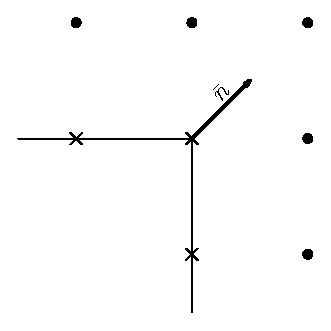
\includegraphics[width=\textwidth]{Figures/free_surface.eps}
%\caption{Free-surface boundary condition represented in the lattice Boltzmann method. 
%Boundary nodes are depicted by crosses, and fluid nodes are represented by dots. One imposes only %phase values at the nodes to calculate laplacians used in the equilibrium functions. In the %population space, one uses the bounce-back rule \cite{yu}, which conserves mass.
%\label{fig:free:surface}}
%\end{figure}

%\begin{figure}
%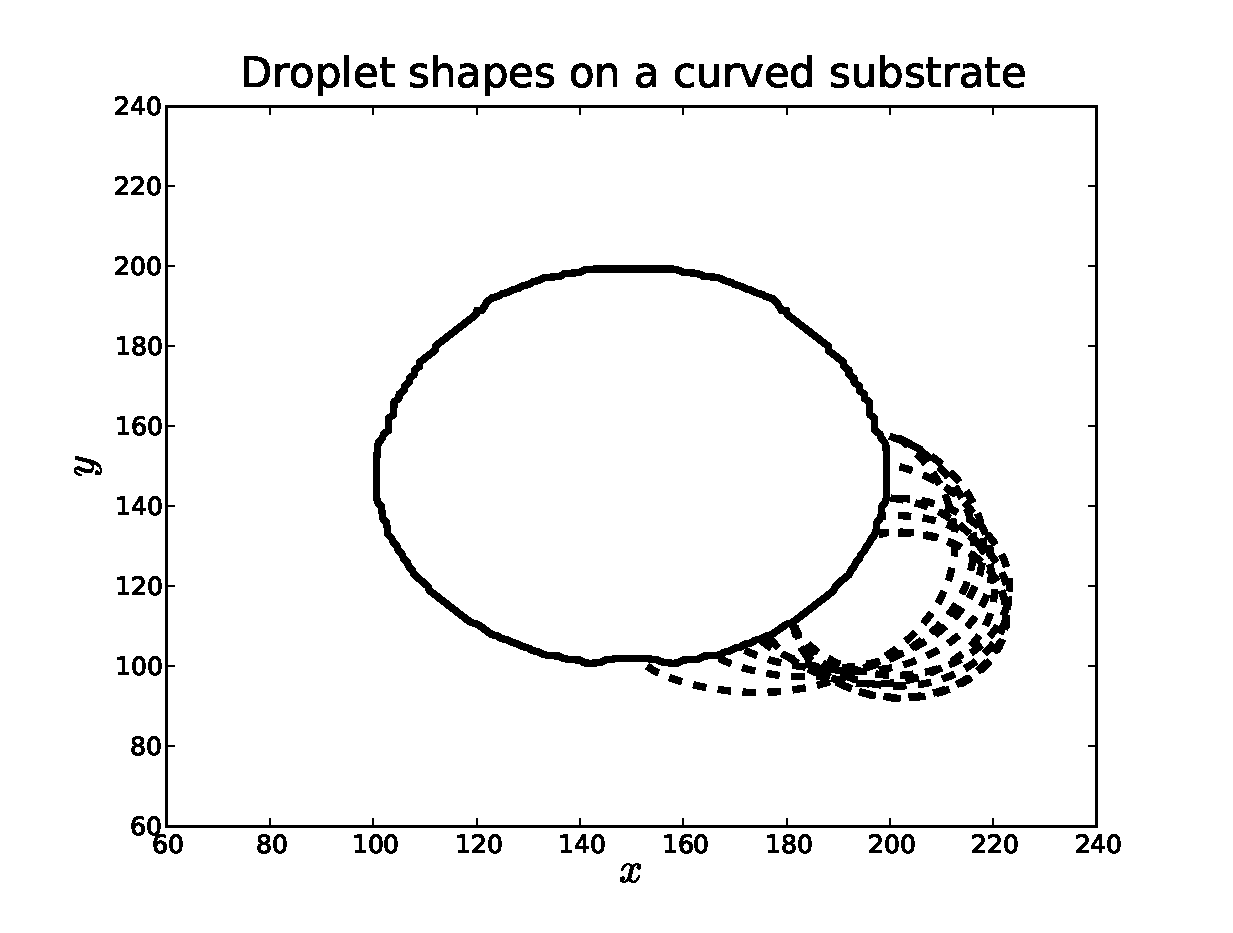
\includegraphics[width=0.5\textwidth]{Figures/droplet_shapes_curved_substrates.eps}
%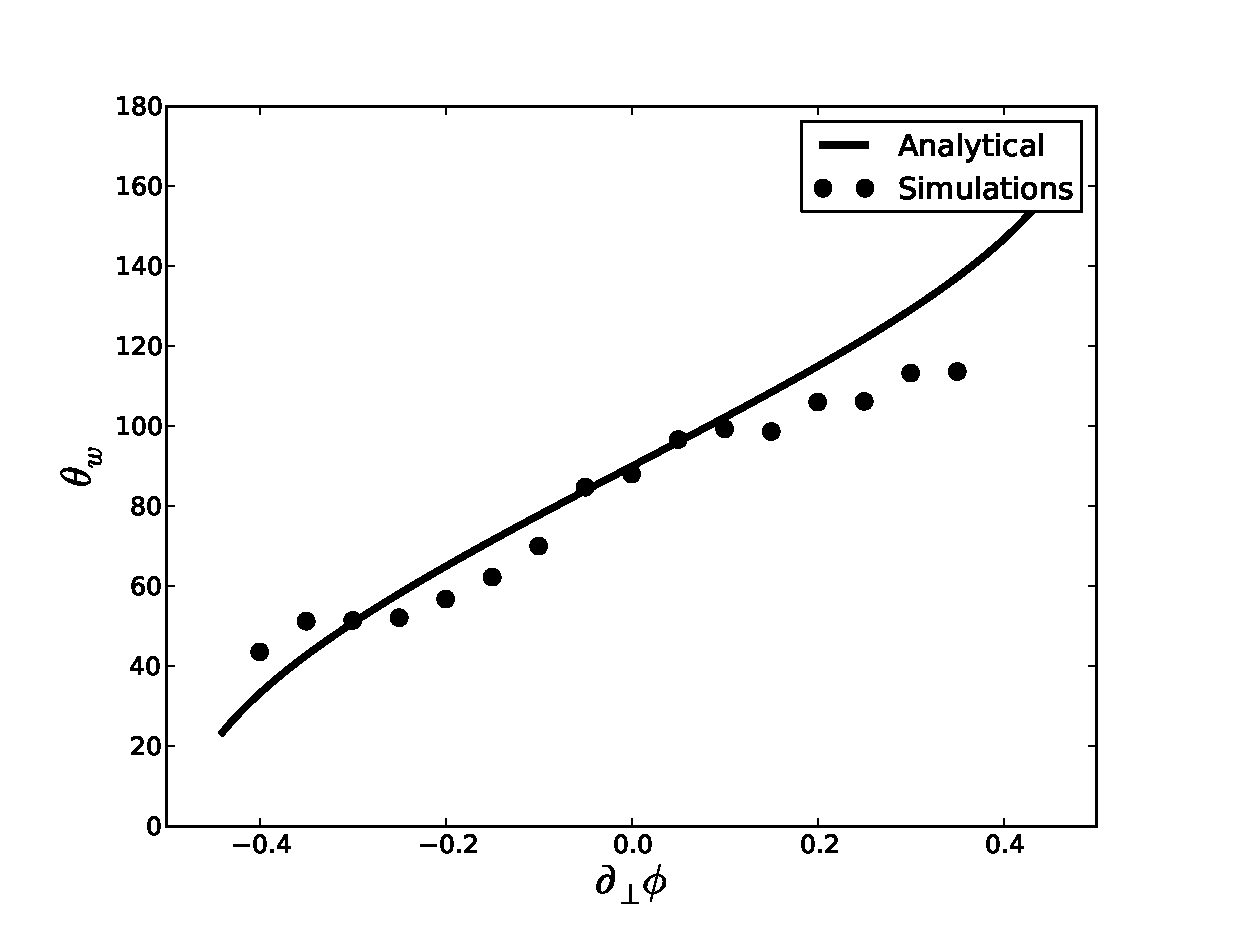
\includegraphics[width=0.5\textwidth]{Figures/main_curve_circle.eps}\\
%\caption{Equilibrium angles at the curved substrate. One can see that the contact angle at the %curved substrate mimics the analytically calculated contact angle at the flat substrate. %\label{fig:equilibrium:droplet:curved}}
%\end{figure}

\section{Results}

\section{Deposition efficiency map}

\section{Conclusions}
The work presented investigates the interaction between emulsion droplets and curved substrates to understand the critical factors controlling the efficiency and the kinetics of the wetting process during collision. We use 2D Lattice Boltzmann methods to simulate spherical emulsion droplets colliding on a curved "cylindrical" substrate. The properties of the substrate are set by controlling its curvature and the three phase contact angle with the emulsion droplet and the surrounding fluid. The emulsion droplet is characterized by its size, viscosity and interfacial tension with the surrounding fluid. As expected we observe that the curvature of the droplet or substrate and the kinetics of the collision process does not effect the equilibrium three phase contact angle after wetting. However a detailed analysis of the collision process reveals that droplets deformation at wetting critically depends on the collision speed and relative dimension of droplet and substrate. Large droplets approaching the substrate very slowly deform very mildly before wetting while during fast collision a higher deformation is achieved before wetting occurs. For small droplets the same trend is found but overall smaller deformation are observed. The results can be rationalized if we consider a hydrodynamic disjoining pressure that retard contact between droplets and substrate. Based on this finding we can map the optimal conditions to achieve successful wetting, deposition and retention of an emulsion droplet on a substrate. This results can be used to guide the design of emulsions used as actives delivery vehicles. Emulsion size and interfacial properties can be tuned to optimize deposition efficiency on the relevant substrates based on the hydrodynamic parameters of the collision process. Such information are of important practical utility in pharmaceutical and cosmetic application in which emulsion droplets are often used to deposit active ingredient on tissues or fibers.  
\bibliographystyle{unsrt}
\bibliography{paper}
\end{document}
